Relacionado a los resultados de cada uno de las ejecuciones del algoritmo, las Figuras \ref{fig:AG_1} a \ref{fig:AG_5} muestran el proceso de convergencia, donde se puede observar que todas las ejecucuciones convergieron en una solución óptima.

\begin{figure}[htbp]
	\centering
	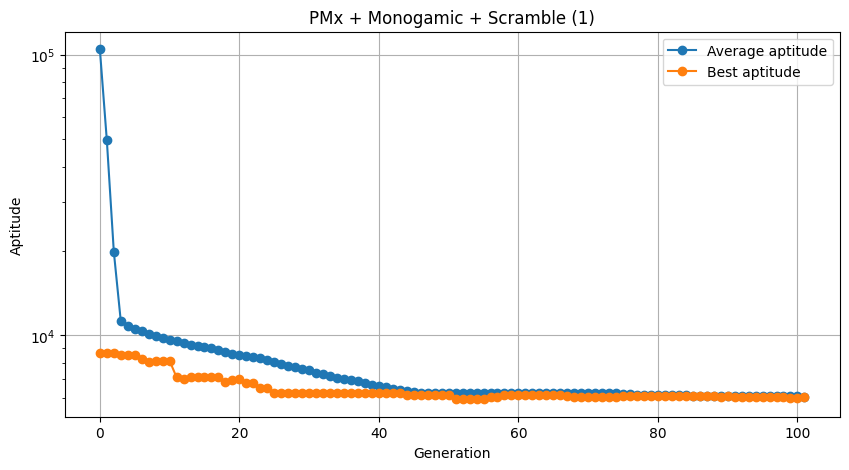
\includegraphics[width=0.6\textwidth]{pmx_monogamic_scramble_(1)}
	\caption{Evolución de la aptitud de los individuos del algoritmo 1.}
	\label{fig:AG_1}
\end{figure}

\begin{figure}[htbp]
	\centering
	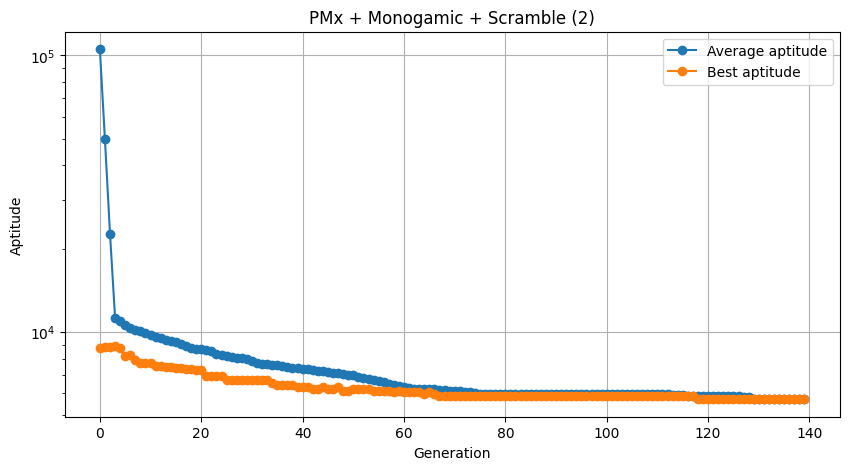
\includegraphics[width=0.6\textwidth]{pmx_monogamic_scramble_(2)}
	\caption{Evolución de la aptitud de los individuos del algoritmo 2.}
	\label{fig:AG_2}
\end{figure}

\begin{figure}[htbp]
	\centering
	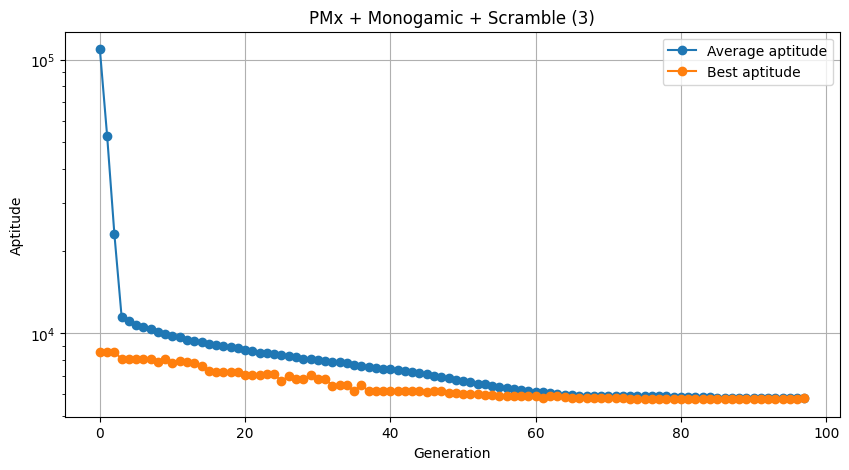
\includegraphics[width=0.6\textwidth]{pmx_monogamic_scramble_(3)}
	\caption{Evolución de la aptitud de los individuos del algoritmo 3.}
	\label{fig:AG_3}
\end{figure}

\begin{figure}[htbp]
	\centering
	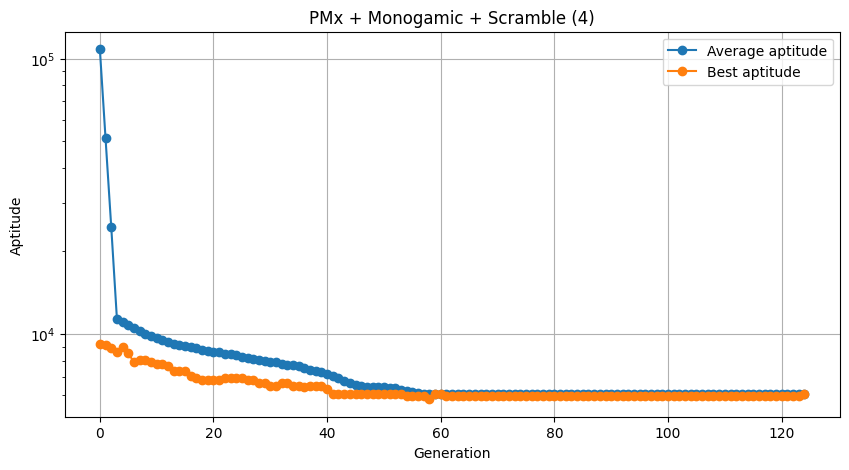
\includegraphics[width=0.6\textwidth]{pmx_monogamic_scramble_(4)}
	\caption{Evolución de la aptitud de los individuos del algoritmo 4.}
	\label{fig:AG_4}
\end{figure}

\begin{figure}[htbp]
	\centering
	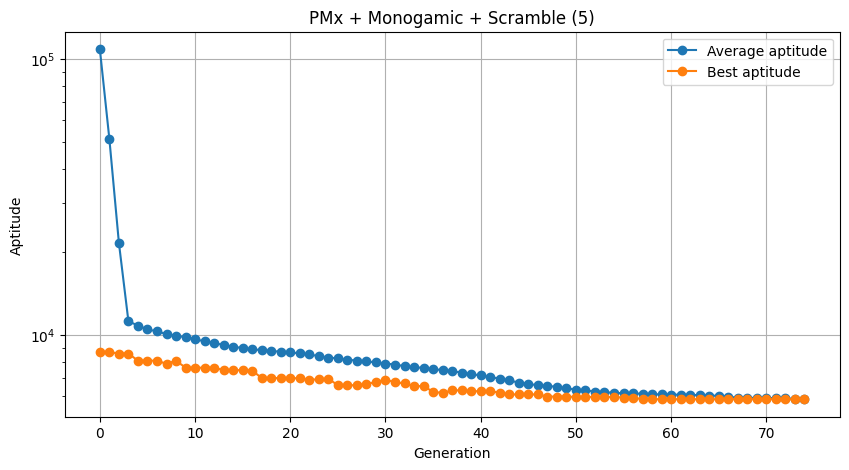
\includegraphics[width=0.6\textwidth]{pmx_monogamic_scramble_(5)}
	\caption{Evolución de la aptitud de los individuos del algoritmo 5.}
	\label{fig:AG_5}
\end{figure}

\FloatBarrier
Relacionado a los resultados finales de cada ejecución, la Tabla \ref{tab:resultados} muestra la distancia obtenida por la mejor ruta de cada ejecución, así como la distancia promedio final. Esto nos da un indicio de la robustez del algoritmo gracias a las pequeñas variaciones entre cada ejecución.

\begin{table}[htbp]
\centering
\caption{Mejores distancias obtenidas en cada ejecución del algoritmo y distancia promedio final.}
\begin{tabular}{ccc}
\hline
\# Ejecución & Menor distancia (km) & Promedio               \\ \hline \hline
1            & 6,057           & \multirow{5}{*}{5,895} \\
2            & 5,707           &                        \\
3            & 5,822           &                        \\
4            & 6,043           &                        \\
5            & 5,846           &                        \\ \hline
\end{tabular}
\label{tab:resultados}
\end{table}